\documentclass[12pt, a4paper]{article}
\usepackage{blindtext}
\usepackage[utf8]{inputenc}
\usepackage{graphicx}
\graphicspath{ {Diagrams/} }

% Title Page
\title{{\Huge PowerEnJoy}}

\author{
	Andrea Battistello
	\\
	William Di Luigi
}


\begin{document}
\maketitle
\tableofcontents



\newpage
\section{Introduction}
	\subsection{Purpose}

	\subsection{Present system}
	
	\subsection{Scope}
	
	\subsection{Goals}

	\subsection{Actors}

	\subsection{Stakeholders}
	
	\subsection{Definitions, acronyms, abbreviations}
	
			\subsubsection{Definitions}
					
			\subsubsection{Acronyms}
				\begin{itemize}
					\item {[PE]} Power EnJoy system
					\item {[PEM]} Power EnJoy Mobile application
				\end{itemize}
					
			\subsubsection{Abbreviations}
					\begin{itemize}
						\item {[Gn]} n-th goal 
						\item {[Dn]} n-th domain assumption
						\item {[Rn.m]} m-th requirement related to goal [Gn]
					\end{itemize}
	
	\subsection{Reference documents}
	
	\subsection{Overview}


\newpage
\section{Overall description}
	\subsection{Product perspective}

	\subsection{Product functions}
		
	\subsection{User characteristics}

	\subsection{Constraints}
	
	\subsection{Assumptions and Dependencies}
	
	\subsection{Future possible implementation}


\newpage
\section{Specific requirements}
	\subsection{External Interface Requirements}
	
	\subsection{Functional requirements / System Functions}
	\subsubsection{Use case diagram}
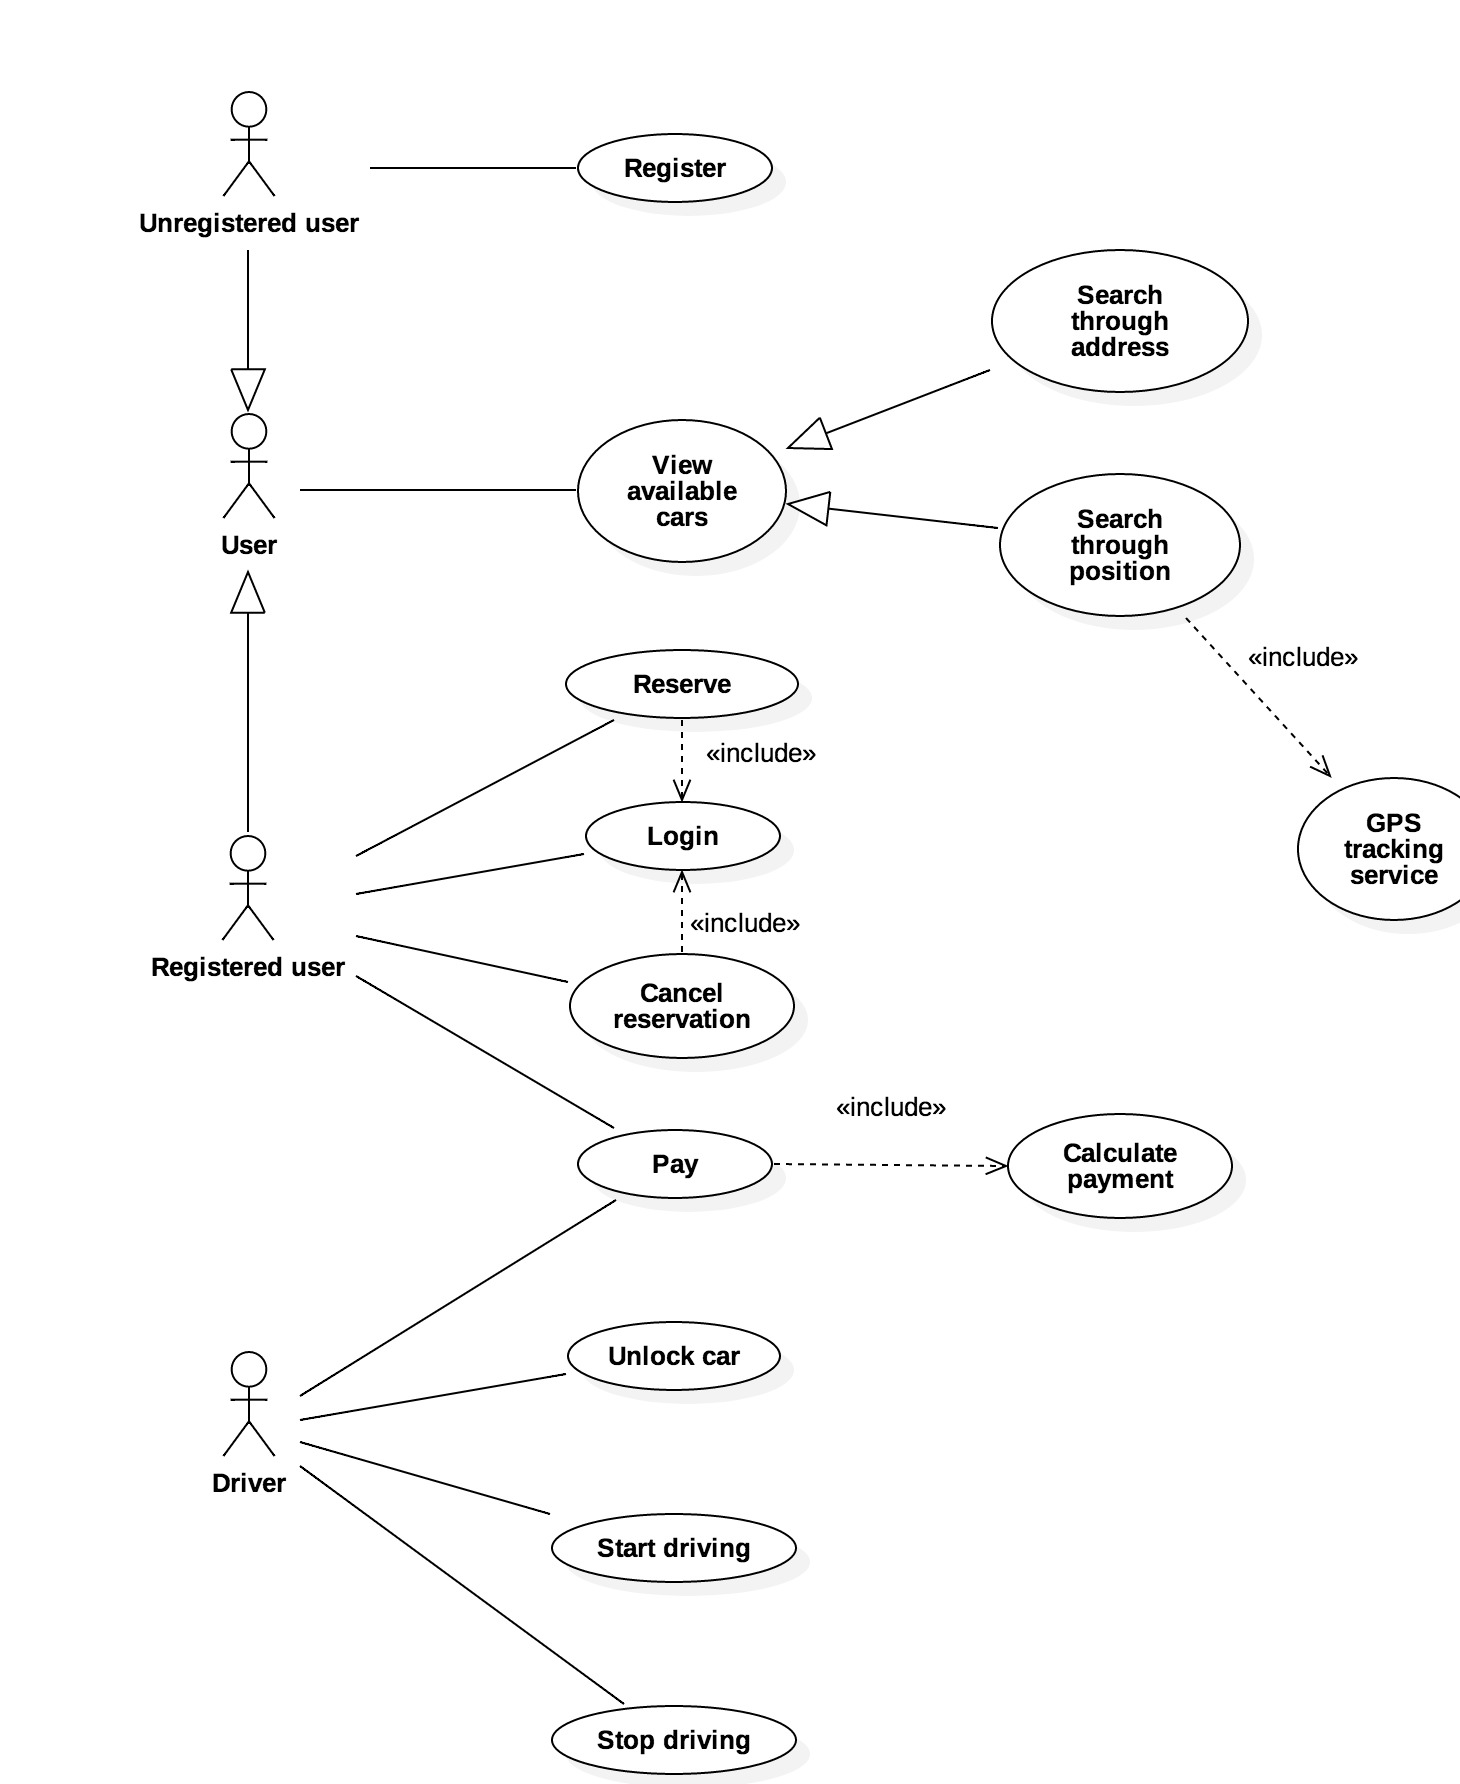
\includegraphics[width=12cm]{UseCaseDiagram1}
	
	\subsection{Scenarios}
	In this section we provide several different scenarios, each of which should clarify how the user interacts with the system in practical situations. 

\subsubsection{Scenario 1 - User registration and login}
Robert is a tech fan and always wants to try out new things. He just discovered PE and immediately downloaded PEM. Next, he inserted both his credentials, payment informations and the numbers of his driving license and his ID card. Robert is also asked to read and accept the terms and conditions. He followed the procedure and after a while he received an email with a password that he must use to access PE system. Robert can now log in with his email and password and search for available cars.

\subsubsection{Scenario 2 - Parking far from recharging station}
Anna is a university student and currently studies abroad. It is a long time she had not seen her parents so she decided to surprise them by getting home. She landed in the nearest airport and took a train to the city. She used PE cars to get home. Unfortunately, her parents' house is far from the city center and the nearest recharging station is 3.5km away. Hence, when she parked the car and finished her run, she received the check with an additional 30\% charge to compensate for the cost required to re-charge the car on-site. 

\subsubsection{Scenario 3 - Recharging the car after use}
Bob is an environmentalist and takes very seriously the issue of climate change. To get around the city he usually uses his electric car but unfortunately he forgot to charge the battery the day before. Hence he used PEM and reserved a car. When he arrived close to the car 15 minutes later, he opened PEM and he sent a notification to the system to unlock the car. Next, he used the car and got to his workplace. He noticed on the car display that the battery level was under 50\%, so he parked close to a recharging station and he plugged the car into the power grid. Soon later, he received the check on his mobile phone with a 30\% discount and an acknowledgment for his good action.

\subsubsection{Scenario 4 - Reservation time expired}
Carl is always in a hurry and hates losing any minute of his precious time. For this reason, he reserved a car through the mobile application while he was still at work, in order to be ready to pick it up 30 minutes later and get home early that day. Unfortunately his boss called him for an unexpected meeting that lasted 2 hours. Carl forgot to cancel his previous reservation, so the system charged him a fee and made the reserved car available again.

\subsubsection{Scenario 5 - Using Power EnJoy with friends}
Dave enjoys going out on Saturday nights and come back home as late as possible with his two friends, Mario and John.  Neither he and his friends has his own car, so they usually use public transportation to get to the pubs. Unfortunately, public transportation service in the city is not available late at night. Therefore, when they wanted to get home, Dave used PEM to reserve the closest car available. When they got in the car, the car detected the additional passengers and informed Dave that a discount would be applied. Dave brought each of his friends at their home and parked the car in a safe area. Soon after he get out the car, he received his check and a notification of the applied discount.

\subsubsection{Scenario 6 - Accidents}
Fred the Trouble Maker is always very unlucky. He signed in the system with his mobile phone and picked up a car to get home. He was happily driving down main street when a truck turned suddenly and struck the car. Fred, luckily undamaged, suddenly phoned to the call center of PE system and reported the accident. After a while, Simon the operator came by and helped Fred with all the required procedure. 

\subsubsection{Scenario 7 - Cancel a reservation}


\subsubsection{Scenario 8 - Web app}
George is out of internet on this mobile phone. Fortunately, he is at home and can log in to PE system through his computer. He found a nearby car available and reserved it. Then, he reached the selected car and sent a SMS with his phone to PE. After a while, the car unlocked and George used it.



	
	\subsection{Class diagram}
	
	\subsection{Other UML diagram / Function sequence diagrams}

	\subsection{Performance requirements}
	
	\subsection{Software system requirements}
	
	\subsection{Alloy}


\newpage
\section{Bibliography}


\end{document}          
